% Slide 27
\begin{frame}{Revisiting the Cliff}
\centering
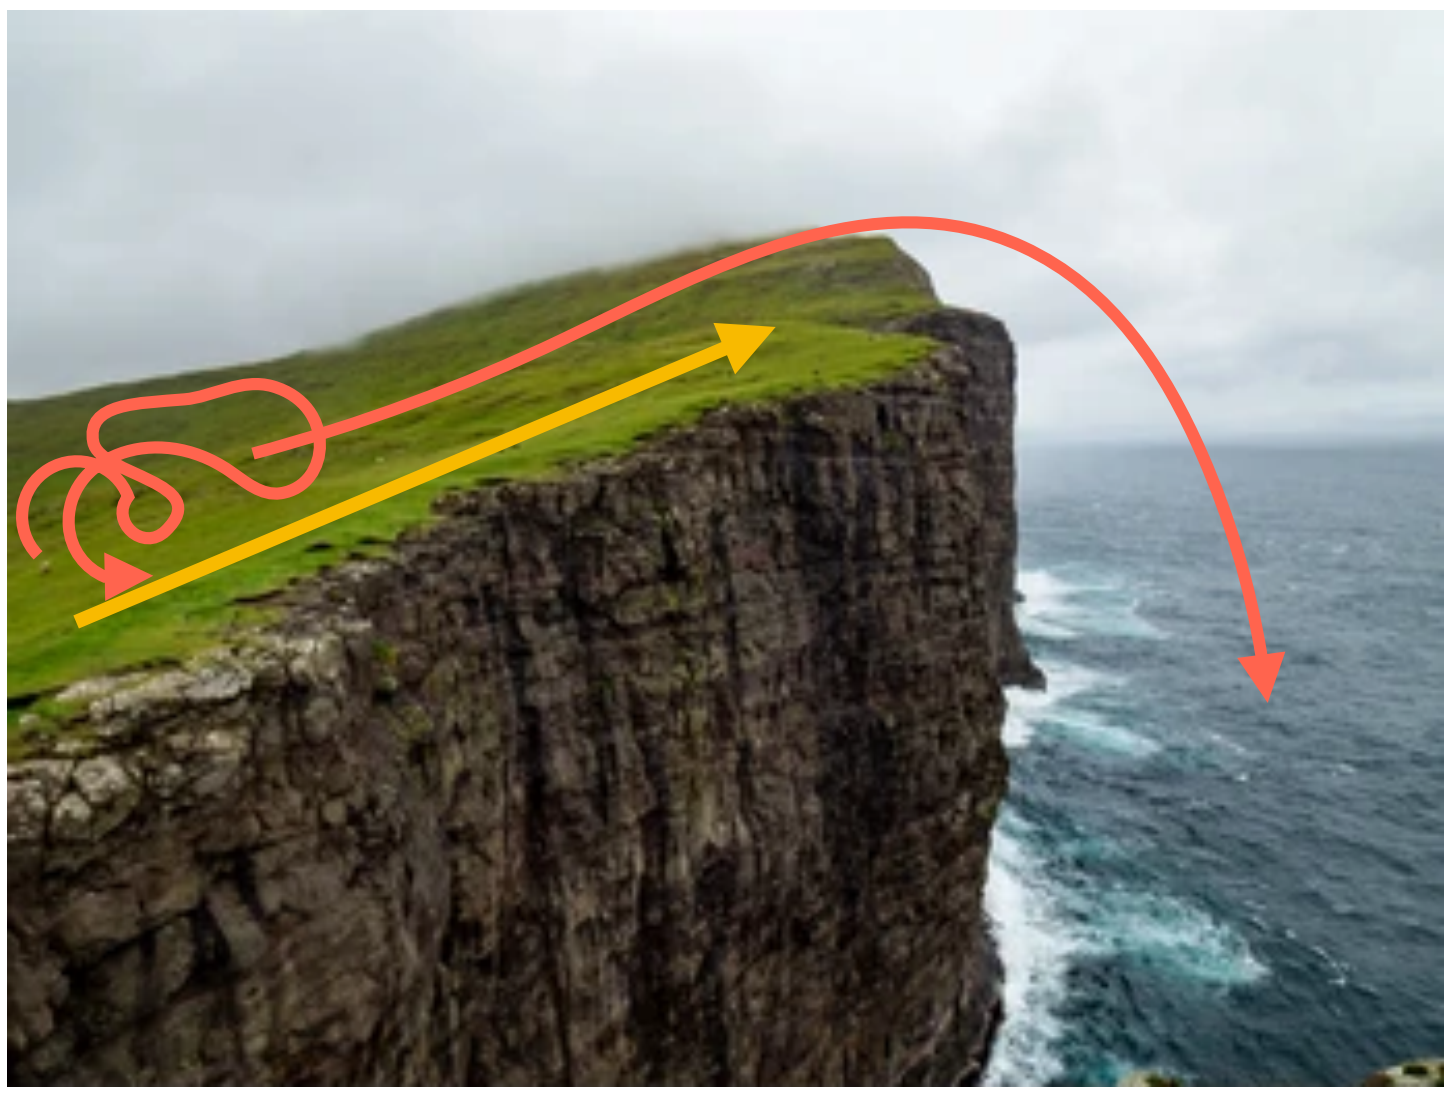
\includegraphics[width=0.42\textwidth]{images/model-based-rl/figures/cliff-revisit.jpg}
\end{frame}

% Slide 28
\begin{frame}{Revisiting the Cliff}
\centering
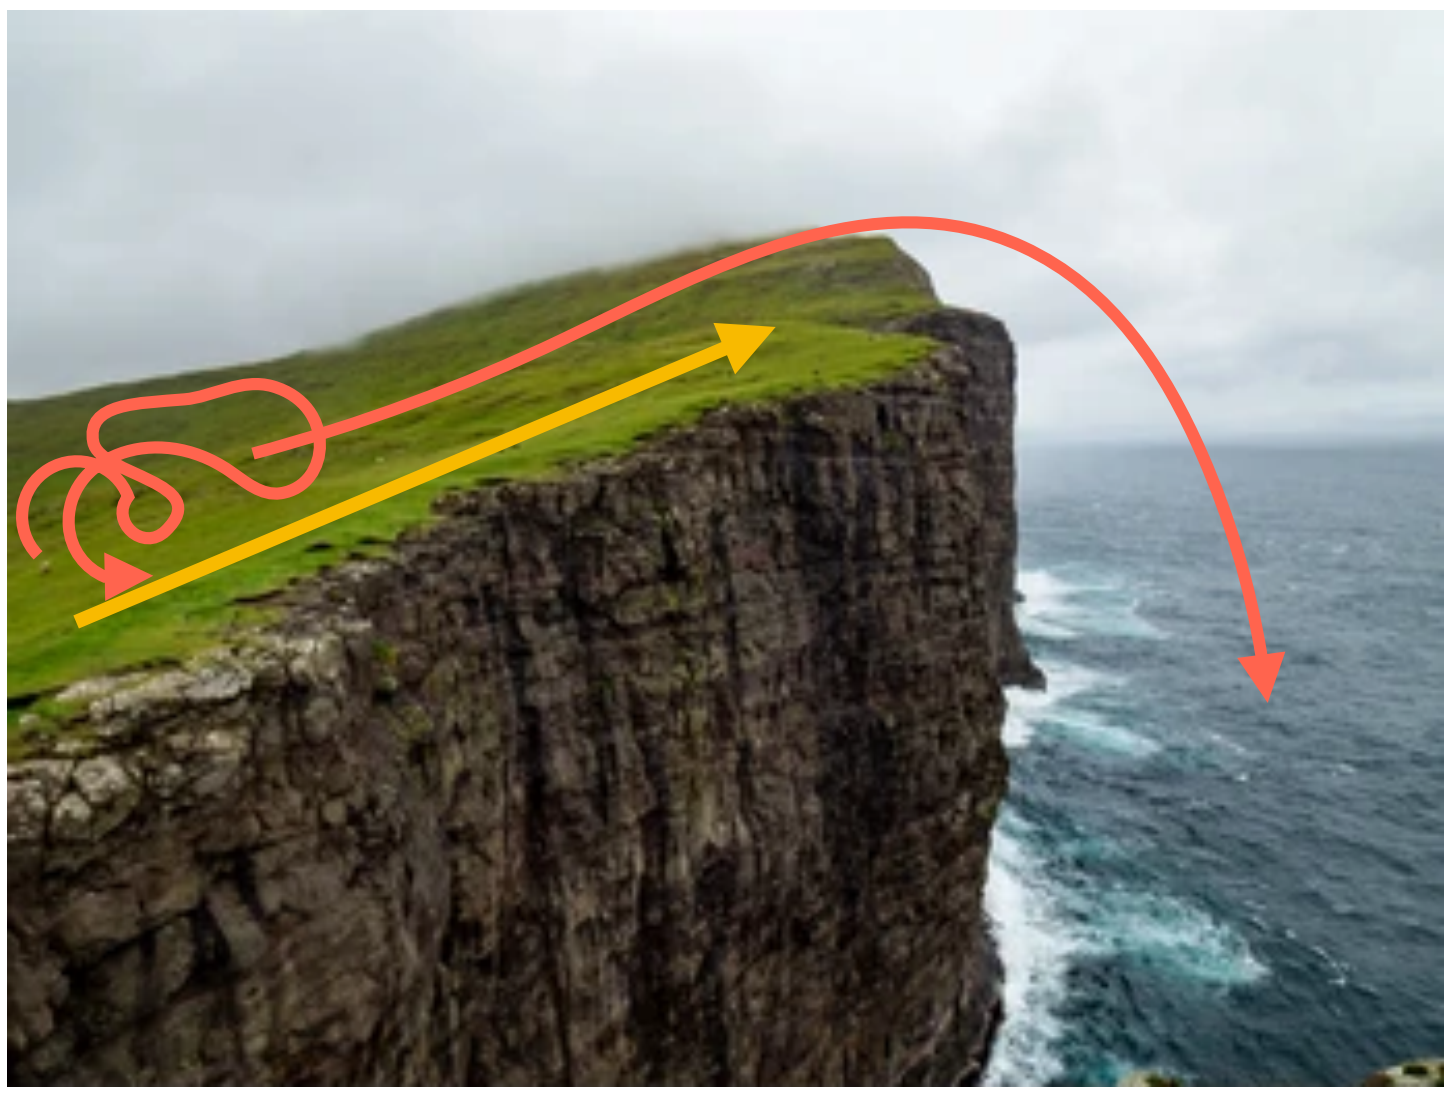
\includegraphics[width=0.36\textwidth]{images/model-based-rl/figures/cliff-revisit.jpg}
\begin{itemize}
    \item Initially, its still the same. The agent learns that going right means
          that we can go higher!
\end{itemize}
\end{frame}

% Slide 29
\begin{frame}{Revisiting the Cliff}
\centering
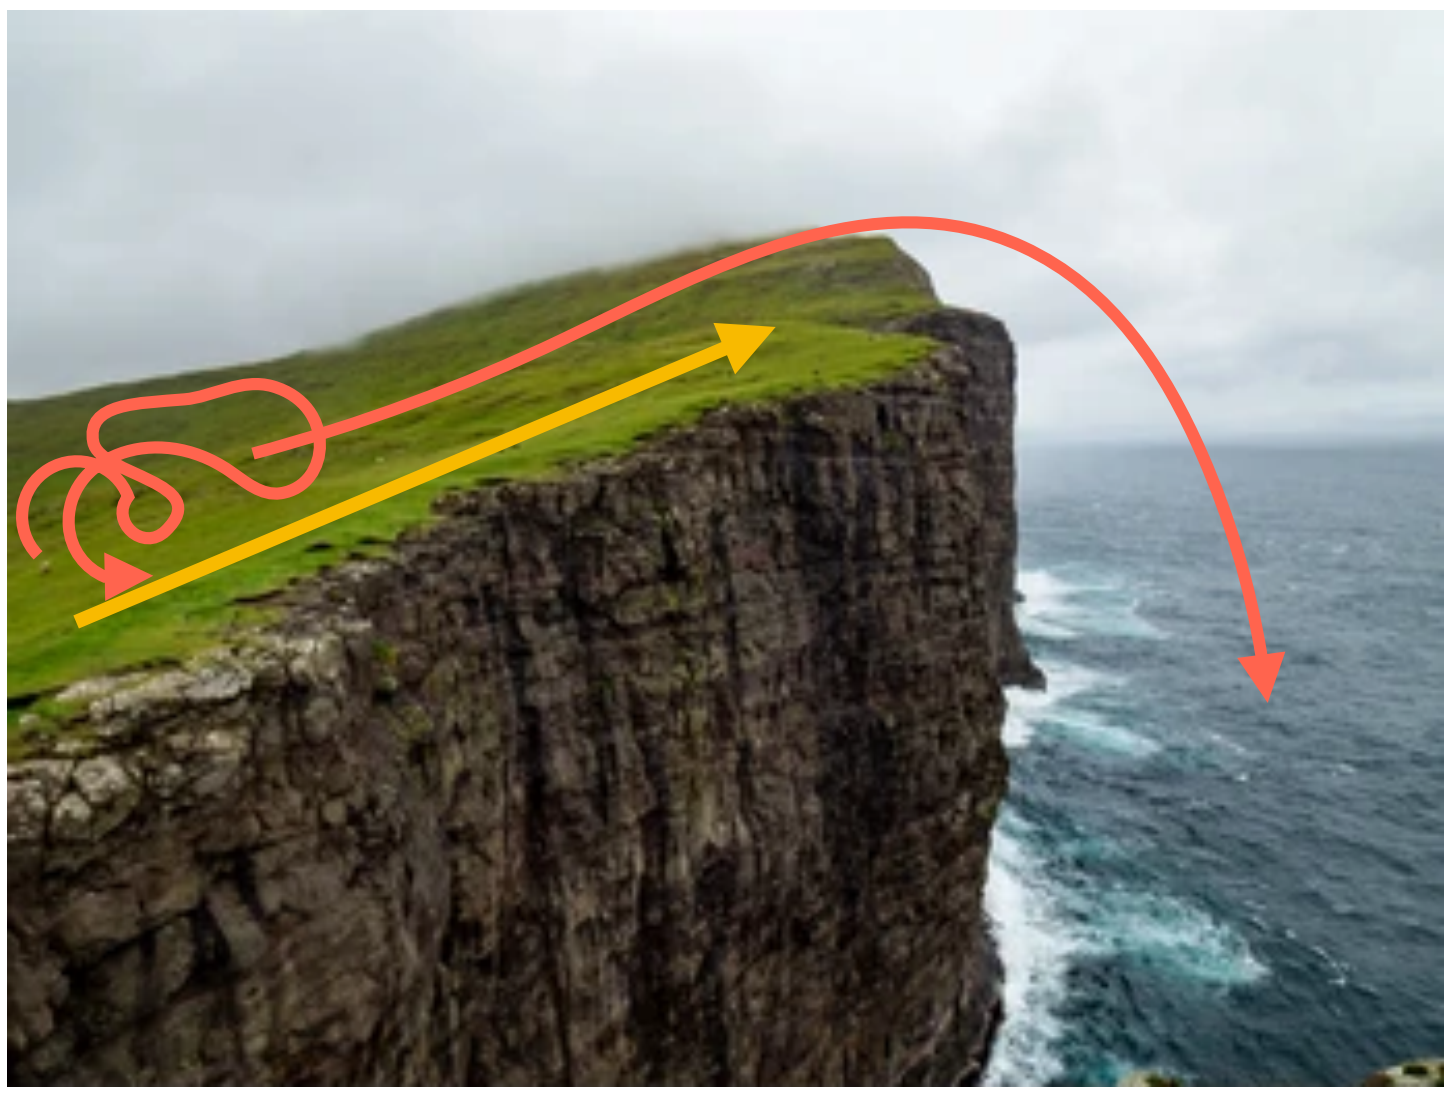
\includegraphics[width=0.36\textwidth]{images/model-based-rl/figures/cliff-revisit.jpg}
\begin{itemize}
    \item Initially, its still the same. The agent learns that going right means
          that we can go higher!
    \item Then we re-train the model using the new observations
\end{itemize}
\end{frame}

% Slide 30
\begin{frame}{Revisiting the Cliff}
\centering
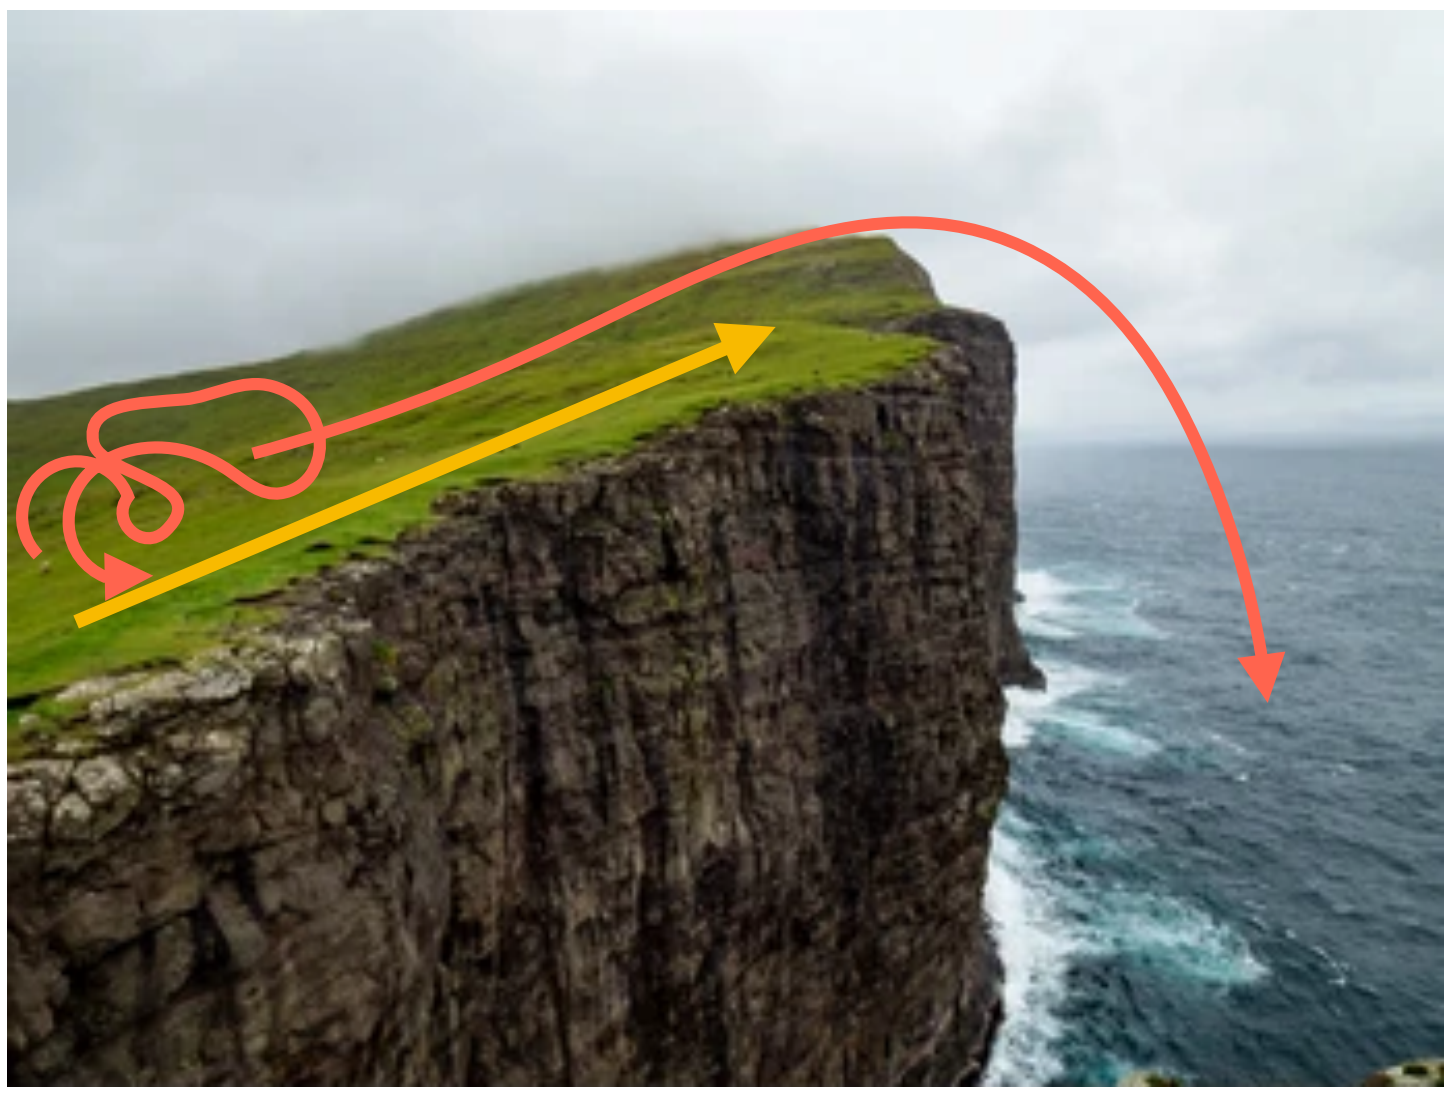
\includegraphics[width=0.36\textwidth]{images/model-based-rl/figures/cliff-revisit.jpg}
\begin{itemize}
    \item Initially, its still the same. The agent learns that going right means
          that we can go higher!
    \item Then we re-train the model using the new observations
    \item The final policy is different now. It learns to go to the top and stop.
\end{itemize}
\end{frame}
